\chapter{Additional features}
\label{chap_add_feat}
%%%%%%%%%%%%%%%%%%%%%%%%%%%%%%%%%%%%%%%%%%%%%%%%%%%%%%%%%%%%%%%%%%%%

\section{Data forwarding}
In order to reduce the number of required stalls in the pipeline and thus improving the efficiency and reducing the average latency of our processor, we have implemented a simple form of data forwarding.
It is important to notice that, after an initial phase of testing without this capability, some additional signals and components have been added to connect some data at different stages of the pipeline. In particular, these are the following:
\begin{itemize}
	\item between \textit{MEM} and \textit{EX} stage
	\item between \textit{WB} and \textit{EX} stage
\end{itemize}

Each of these signals goes through a different multiplexer, which select either this data or the data coming from the previous stage. This selection is made by checking the destination and the source registers of two following instructions. When we have that
\[R^{i-1}_{dest}\quad = \quad R^{i}_{sorce}\]
then the signal coming from the subsequent stage is selected.


\section{Dynamic branch prediction}
\label{dyn_br}
In order not to waste too much clock cycles waiting for the correct value of the \textit{PC} register, we have designed a unit that provides a dynamic prediction regarding a branch instruction. In particular, it is possible, with a defined value of the \textit{PC} corresponding to a branch, to get whether is a better speculation to take or not to take the branch, while waiting for the correct \textit{PC}, which comes after the execution stage. 
There are actually 16 possible entries in our branch. Each of them is composed 
by a part of the \pc and a prediction state, represented on two bits, as 
reported in table \ref{pred_tab}. Every time a new instruction is issued, this 
entity checks whether it is a branch type or not. If so, the bits from 5 to 2 
of the \pc related to the instruction are taken into account as address to the 
table, as shown in figure \ref{bht_fig}. At this point, the content of this 
location is checked:
\begin{itemize}
	\item if the value stored corresponds to the \pc, then the prediction contained is the one related to thie current instruction, and therefore it can be freely used
	\item if not, the previously stored value is overwritten, as long as its prediction: the current prediction is set to a "weakly not taken case"
\end{itemize}

\begin{table}[]
	\centering
	\begin{tabular}{l|cccc}
		\toprule
		& 00        & 01      & 10     & 11       \\
		\toprule
		Encoding     & Strong NT & Weak NT & Weak T & Strong T \\
		\midrule
		NS when HIT  & 00        & 00      & 11     & 11       \\
		NS when MISS & 01        & 10      & 01     & 10      	\\
		\bottomrule
	\end{tabular}
\caption{Possible states for predictor}
\label{pred_tab}
\end{table}


\begin{figure}
	\centering
	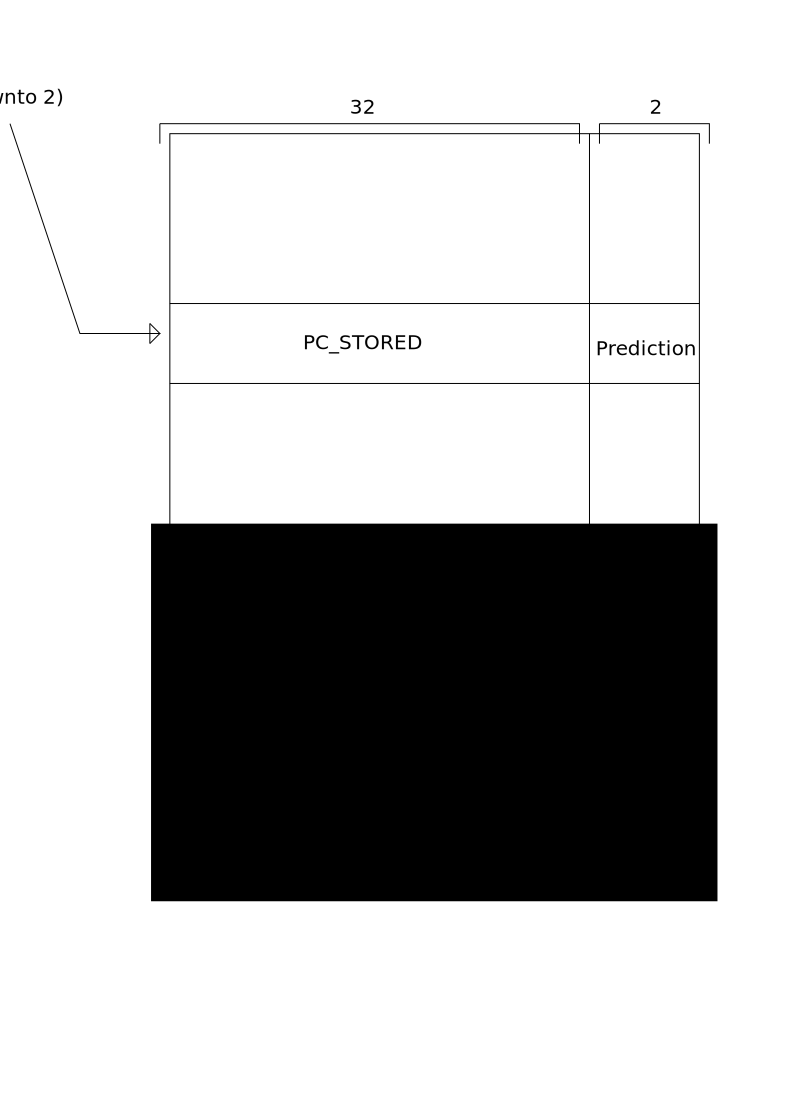
\includegraphics[scale=0.5]{chapters/figures/bht}
	\caption{Schematic for BHT}
	\label{bht_fig}
\end{figure}